%-*-latex-*-
\sectionthree{Heap and complete trees}
\begin{python0}
from solutions import *; clear()
\end{python0}

Recall that we have complete freedom in choosing where to insert a new node.
We also have complete freedom in choosing any leaf to use to overwrite
a node to be deleted as long as the leaf is a descendent of the node whose
value is to delete.
In particular, if we are remove the value of the root of the heap,
we can choose any leaf.

It's because of the above,
after every insert and root value removal,
we can alway ensure that the heap is complete.
Recall that a complete binary tree that is almost full except that the
last level might not have all the leaves.
are at the same level.
Furthermore, we can force to have
all the leaves at the last level to be all on the left side of the whole
tree.
This is what I mean by \lq\lq left side'' of the tree:


\begin{center}

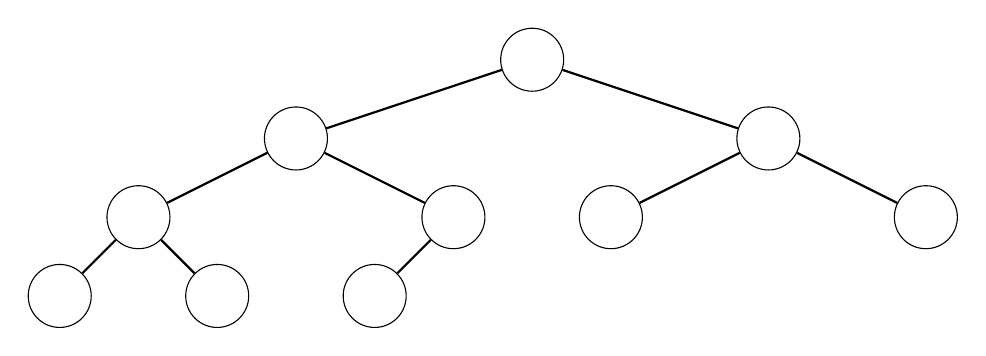
\begin{tikzpicture}
\node at (6,-1) [circle,draw,minimum size=8mm] (A) {};
\node at (3,-2) [circle,draw,minimum size=8mm] (B) {};
\node at (9,-2) [circle,draw,minimum size=8mm] (C) {};
\node at (1,-3) [circle,draw,minimum size=8mm] (D) {};
\node at (5,-3) [circle,draw,minimum size=8mm] (E) {};
\node at (7,-3) [circle,draw,minimum size=8mm] (F) {};
\node at (11,-3) [circle,draw,minimum size=8mm] (G) {};
\node at (0,-4) [circle,draw,minimum size=8mm] (H) {};
\node at (2,-4) [circle,draw,minimum size=8mm] (I) {};
\node at (4,-4) [circle,draw,minimum size=8mm] (J) {};
\draw [-,thick] (A) -- (B);
\draw [-,thick] (A) -- (C);
\draw [-,thick] (B) -- (D);
\draw [-,thick] (B) -- (E);
\draw [-,thick] (C) -- (G);
\draw [-,thick] (C) -- (F);
\draw [-,thick] (D) -- (H);
\draw [-,thick] (D) -- (I);
\draw [-,thick] (E) -- (J);

;
\end{tikzpicture}
    
\end{center}



This can be achieved by
\begin{tightlist}
\li During insert, always insert a leaf just to the right of the
rightmost leaf at the last level.
\li During delete, always using the right most leaf of the 
last level whenever we remove the root.
\end{tightlist}





\begin{ex} 
  \label{ex:some-decision1}
  \tinysidebar{\debug{exercises/{empty0/question.tex}}}
  \solutionlink{sol:some-decision1}
  \qed
\end{ex} 
\begin{python0}
from solutions import *
add(label="ex:some-decision1",
    srcfilename='exercises/some-decision1/answer.tex') 
\end{python0}



\begin{ex} 
  \label{ex:some-decision1}
  \tinysidebar{\debug{exercises/{empty0/question.tex}}}
  \solutionlink{sol:some-decision1}
  \qed
\end{ex} 
\begin{python0}
from solutions import *
add(label="ex:some-decision1",
    srcfilename='exercises/some-decision1/answer.tex') 
\end{python0}



\begin{ex} 
  \label{ex:some-decision1}
  \tinysidebar{\debug{exercises/{empty0/question.tex}}}
  \solutionlink{sol:some-decision1}
  \qed
\end{ex} 
\begin{python0}
from solutions import *
add(label="ex:some-decision1",
    srcfilename='exercises/some-decision1/answer.tex') 
\end{python0}


Being complete means that the heaps can have the minimal possible height.
At this point, you ought to know that this is a good thing.

This also implies right away that the worse runtimes for 
insert and delete is $O(\log n)$ for both insert and delete
as long as we keep the heap complete.

